\documentclass[12pt]{report}
%\documentclass[12pt, draft]{report}
\usepackage[a3paper]{geometry}
\usepackage{multirow}
\usepackage{graphicx}
\usepackage{color}
\usepackage{hyperref}
\usepackage{enumerate}
\usepackage{amsthm}
\usepackage{amssymb}
\usepackage{listings}
\usepackage{pdflscape}
\usepackage{color, colortbl}
\usepackage[table]{xcolor}
\usepackage{longtable}
\usepackage{tabularx}
\geometry{total={297mm, 420mm}, left=20mm, right=22mm, top=25mm, bottom=25mm}

\hypersetup{
    pdffitwindow=true,
    pdfstartview={FitH},
    colorlinks=true,
    linkcolor=blue,
    citecolor=red,
    urlcolor=blue
}

\lstset{
    basicstyle=\footnotesize,
    numbers=left,
    numberstyle=\footnotesize,
    stepnumber=1,
    numbersep=5pt,
    frame=single,
    breaklines=true,
    title=\lstname
}

\sloppy
\newtheorem{definition}{Definition}

\begin{document}
\author{Krzysztof Jusiak}
\title{C++ FSM frameworks comparison}
\frenchspacing
\maketitle

\begin{abstract}
Document presents comparison between C++ FSM frameworks:
\begin{itemize}
\item Boost Meta State Machine (msm)
\item Boost State Chart (statechart)
\item Quick Finite State Machine (QFsm)
\end{itemize}
\end{abstract}

\clearpage
\tableofcontents

\chapter{Introduction}

\section{Finite state machine}
\textbf{Unified Modeling Language} is a standardized general-purpose modeling language in the field of object-oriented software engineering. The standard is managed, and was created by, the Object Management Group.\\
\url{http://www.omg.org/spec/UML}\\

\textbf{State diagram} is a type of diagram used in computer science and related fields to describe the behavior of systems. State diagrams require that the system described is composed of a finite number of states; sometimes, this is indeed the case, while at other times this is a reasonable abstraction. There are many forms of state diagrams, which differ slightly and have different semantics.\\
\url{http://en.wikipedia.org/wiki/State\_diagram}\\

\textbf{Finite state machine} is a mathematical abstraction sometimes used to design digital logic or computer programs. It is a behavior model composed of a finite number of states, transitions between those states, and actions, similar to a flow graph in which one can inspect the way logic runs when certain conditions are met. It has finite internal memory, an input feature that reads symbols in a sequence, one at a time without going backward; and an output feature, which may be in the form of a user interface, once the model is implemented. The operation of an FSM begins from one of the states (called a start state), goes through transitions depending on input to different states and can end in any of those available, however only a certain set of states mark a successful flow of operation (called accept states).\\
\url{http://en.wikipedia.org/wiki/Finite-state\_machine}\\

\begin{figure}[htbp]
    \centering
    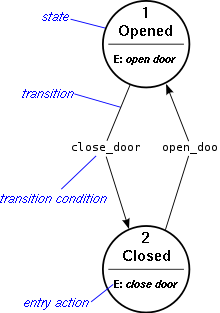
\includegraphics[scale=0.8]{images/fsm.png}
    \caption[FSM]{FSM}
\end{figure}

\textbf{The Domain Abstraction} ion of finite state machines consists of three simple elements.
\begin{itemize}
\item \textbf{States}\\
    An FSM must always be in one of several well-defined states. For example,
    the states of a simple CD player might be called Open, Empty, Stopped (with
    a CD in the drawer), Paused, and Playing. The only persistent data
    associated with a pure FSM is encoded in its state, though FSMs are seldom
    used alone in any system. For example, the parsers generated by YACC are
    built around a stack of state machines; the state of the whole system includes
    that of the stack and of each FSM in the stack.
\item \textbf{Events}\\
    State changes are triggered by events. For example in CD player example, most
    events would correspond to button presses on its front panel: play, stop,
    pause, and open/close (the button that opens and closes the drawer). Events
    aren't necessarily "pushed" into a state machine from the outside, though.
    For example, in YACC parsers, each event represents a different token, and
    is "pulled" from the input stream by the parsing process. In some systems,
    events contain associated data. For instance, an identifier token in a C++
    parser might carry the text of the identifier, while an integer-literal token
    might carry the value of the integer.
\item \textbf{Transitions}\\
    Each state can have any number of transitions to other states. Each transition
    is labeled with an event. To process an event, the FSM follows the transition
    that starts from the current state and is marked with that event. For example,
    a CD player has a transition from Playing to Stopped labeled with the stop
    event. Usually, transitions also have some associated action, such as stop
    playback in the case of our CD player. In the case of YACC, following
    transitions means manipulating the stack of FMSs and/or executing the user's
    semantic actions.
\end{itemize}

\textbf{State transition table} is a table showing what state (or states in the case of a nondeterministic finite automaton) a finite semiautomaton or finite state machine will move to, based on the current state and other inputs. A state table is essentially a truth table in which some of the inputs are the current state, and the outputs include the next state, along with other outputs.\\
\url{http://en.wikipedia.org/wiki/State\_transition\_table}\\

\begin{figure}[htbp]
    \centering
    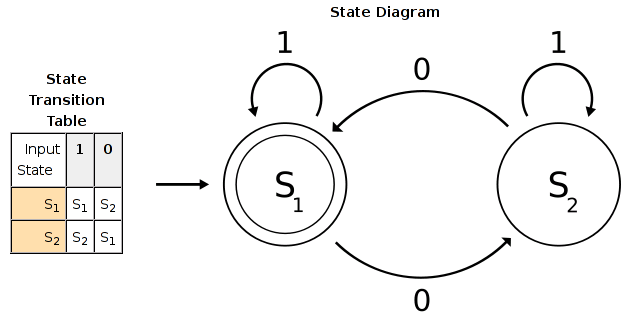
\includegraphics[scale=0.6]{images/transition_table.png}
    \caption[State transition table]{State transition table}
\end{figure}

\textbf{Virtual finite state machine} is a finite state machine (FSM) defined in a virtual environment. The VFSM concept provides a software specification method to describe the behaviour of a control system using assigned names of input control properties and of output actions. The behaviour specification is built by a state table which describes all details of a single state of the VFSM.\\
\url{http://en.wikipedia.org/wiki/VFSM}\\

\begin{figure}[htbp]
    \centering
    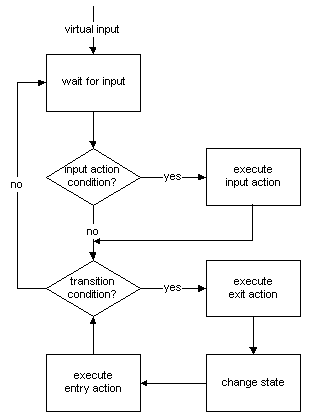
\includegraphics[scale=0.8]{images/vfsm.png}
    \caption[VFSM]{VFSM}
\end{figure}

\newpage
\textbf{State table} defines all details of the behaviour of a state of a VFSM. It consists of three columns: in the first
column state names are used, in the second the virtual conditions built out of input names using the positive logic
algebra are placed and in the third column the output names appear.\\

\begin{figure}[htbp]
    \centering
    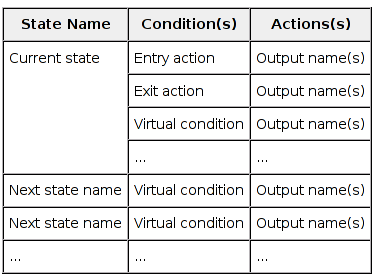
\includegraphics[scale=0.8]{images/state_table.png}
    \caption[State table]{State table}
\end{figure}

Read the table as following: the first two lines define the entry and exit actions of the current state. The following
lines which do not provide the next state represent the input actions. Finally the lines providing the next state
represent the state transition conditions and transition actions. All fields are optional. A pure combinatorial VFSM is
possible in case only where input actions are used, but no state transitions are defined. The transition action can be
replaced by the proper use of other actions.\\


\section{C++ FSM Frameworks}

\subsection{FSM framework implementation}
Some basic concepts how FSM might be realized due to:

\begin{itemize}
\item Concept
    \begin{itemize}
        \item Declarative - transitions are declared at the beginning and can't be changed
        \item Imperative - transitions could have happens in custom handling on event
    \end{itemize}

\item Approach
    \begin{itemize}
        \item Compile time - transitions declared during compile time
        \item Run time - transitions declared during run time
    \end{itemize}

\item Data
    \begin{itemize}
        \item FSM driven - data in FSM
        \item State driven - data in states
        \item Action driven - data in actions
    \end{itemize}
\end{itemize}

\subsection{State machine example}
To visualize differences between frameworks small example was introduced
and implemented in all frameworks. State machine \textit{Player} contains 2 states \textit{Open and Close}.
Event \textit{OpenClose} trigger transition to the next state
(alternately \textit{Open and Close}).

\begin{figure}[htbp]
    \centering
    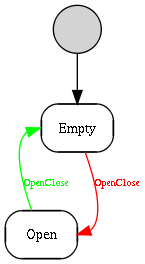
\includegraphics[scale=0.8]{images/simple.png}
    \caption[Simple state machine]{Simple state machine}
\end{figure}

\begin{enumerate}
\item \textbf{Boost Meta State Machine} (MSM)\\
\url{http://www.boost.org/doc/libs/1\_47\_0/libs/msm/doc/HTML/index.html}
\begin{itemize}
\item \textbf{Concept} Declarative
\item \textbf{Approach} Compile time
\item \textbf{Data} State driven, FSM driven
\end{itemize}
\lstinputlisting[language=C++]{frameworks/msm.hpp}

\newpage
\item \textbf{Boost State Chart} (StateChart)\\
\url{http://www.boost.org/doc/libs/1\_47\_0/libs/statechart/doc/index.html}
\begin{itemize}
\item \textbf{Concept} Declarative, Imperative
\item \textbf{Approach} Compile time, Run time
\item \textbf{Data} State driven
\end{itemize}

\lstinputlisting[language=C++]{frameworks/statechart.hpp}

\item \textbf{Quick Finite State Machine} (QFsm)
\begin{itemize}
\item \textbf{Concept} Declarative
\item \textbf{Approach} Compile time
\item \textbf{Data} Action driven
\end{itemize}
\lstinputlisting[language=C++]{frameworks/qfsm.hpp}

\end{enumerate}


\chapter{FSM Comparison}
\section{FURPS}

\textbf{FSM Framework Design Goals}
\begin{itemize}
\item \textbf{Interoperability}\\
    State machines are typically just an abstraction for describing the logic of a system
    targeted at some problem domain(s) other than FSM construction. We'd like to be able to use libraries
    built for those domains in the implementation of our FSMs, so we want to be sure we can comfortably
    interoperate with other DSELs.

\item \textbf{Declarativeness}\\
    State machine authors should have the experience of describing the structure of
    FSMs rather than implementing their logic. Ideally, building a new state machine should involve little
    more than transcribing its stat transition table into a C++ program. As framework providers, we should be able to
    seamlessly change the implementation of a state machine's logic without affecting the author's
    description.

\item \textbf{Expressiveness}\\
    It should be easy both to represent and to recognize the domain abstraction in a
    program. In our case, an state transitoin table in code should look very much as it does when we design a state
    machine on paper.

\item \textbf{Efficiency}\\
    A simple FSM should ideally compile down to extremely tight code
    that can be optimized into something appropriate even for a tiny embedded system. Perhaps more
    importantly, concerns about the efficiency of our framework should never give programmers an
    excuse for using ad hoc logic where the sound abstraction of a finite state machine might otherwise
    apply.

\item \textbf{Static Type Safety}\\
    It's important to catch as many problems as possible at compile time. A typical
    weakness of many traditional FSM designs is that they do most of their checking at
    runtime. In particular, there should be no need for unsafe downcasts to access the different datatypes
    contained by various events.

\item \textbf{Maintainability}\\
    Simple changes to the state machine design should result in only simple changes to
    its implementation. This may seem like an obvious goal, but it's nontrivial to attainexperts have tried
    and failed to achieve it. For example, when using the State design pattern, a single change
    such as adding a transition can lead to refactoring multiple classes.

\item \textbf{Scalability}\\
    FSMs can grow to be really complex, incorporating
    such features as per-state entry and exit actions, conditional transition guards, default and triggerless
    transitions and even sub-states. If the framework doesn't support these features today, it should be
    reasonably extensible to do so tomorrow.
\end{itemize}

\newpage
\textbf{FURPS} is an acronym representing a model for classifying software quality attributes (functional and non-functional requirements):
\begin{itemize}
\item \textbf{F}unctionality - Feature set, Capabilities, Generality, Security
\item \textbf{U}sability - Human factors, Aesthetics, Consistency, Documentation
\item \textbf{R}eliability - Frequency/severity of failure, Recoverability, Predictability, Accuracy, Mean time to failure
\item \textbf{P}erformance - Speed, Efficiency, Resource consumption, Throughput, Response time
\item \textbf{S}upportability - Testability, Extensibility, Adaptability, Maintainability, Compatibility, Configurability, Serviceability, Installability, Localizability, Portability
\end{itemize}

\subsection{FURPS and FSM Frameworks}

\begin{itemize}
\item \textbf{Functionality}
    \begin{enumerate}[a)]
        \item UML features / extensions
            \begin{itemize}

                \item State machine
                    \begin{itemize}
                        \item Nested FSMs
                        \item Orthogonal regions
                        \item Shallow history
                        \item Deep history
                    \end{itemize}

                \item States
                    \begin{itemize}
                        \item Normal state
                        \item Initial state
                        \item Final state
                        \item Super state
                        \item Pseudo state
                    \end{itemize}

                \item Events
                    \begin{itemize}
                        \item Call event
                        \item Internal event
                    \end{itemize}

                \item Reactions
                    \begin{itemize}
                        \item Guard
                        \item Transition
                        \item Deferral
                        \item Completion/Anonymous transition
                        \item Internal transition
                        \item Self transition
                        \item Conflicting transition (overlapping guards, internal transition in sub fsm and other state)
                    \end{itemize}

                \item Actions
                    \begin{itemize}
                        \item Entry action
                        \item Exit action
                        \item Transition action
                    \end{itemize}

            \end{itemize}

        \item Extra features
            \begin{itemize}
                \item Logging (frameworks supports logging events)
            \end{itemize}
    \end{enumerate}

\item \textbf{Usability}
    \begin{enumerate}[a)]
        \item User interface
            \begin{itemize}
                \item Simple
                \item Intuitive
                \item Not redundant
            \end{itemize}
    \end{enumerate}

\item \textbf{Repeatability}
    \begin{enumerate}[a)]
        \item Exception safety
    \end{enumerate}

\item \textbf{Performance}
    \begin{enumerate}[a)]
        \item Event processing (dispatching) time
        \item Binary size (debug, release)
        \item Runtime memory consumption (valgrind)
        \item Compilation time
    \end{enumerate}

\item \textbf{Supportability}
    \begin{enumerate}[a)]
        \item Testability (dependency injection)
    \end{enumerate}

\item \textbf{Others}
    \begin{enumerate}[a)]
        \item UML compatibility
        \item UML state diagram generation (how easy is to generate state diagram / scripts existence)
    \end{enumerate}

\end{itemize}
\begin{table}[ht]

\newcommand{\yes}{\cellcolor{green}\checkmark}
\newcommand{\simple}{\cellcolor{green}simple}
\newcommand{\some}{\cellcolor{yellow}no superstate}
\newcommand{\no}{\cellcolor{red}-}
\newcommand{\verify}{\cellcolor{yellow}?}
\newcommand{\x}{\cellcolor{white}x}
\newcommand{\notall}{\cellcolor{orange}not all}

\caption{FURPS FSM comparison}
\centering
\begin{tabular}{| l | l | c | c | c | c | c |}
\hline
FURPS &                             & MSM       & StateChart    & QFsm       \\
\hline
\multirow{6}{*}{State machine}
& Nested FSMs                       & \yes      & \yes          & \yes       \\
& Orthogonal regions                & \yes      & \yes          & \yes       \\
& Shallow history                   & \yes      & \yes          & \yes       \\
& Deep history                      & \yes      & \yes          & \yes       \\
\hline
\multirow{5}{*}{States}
& Normal state                      & \yes      & \yes          & \yes       \\
& Initial state                     & \yes      & \yes          & \yes       \\
& Final state                       & \yes      & \yes          & \yes       \\
& Super state                       & \no       & \no           & \no        \\
& Pseudo state                      & \yes      & \no           & \yes       \\
\hline
\multirow{3}{*}{Events}
& Call event                        & \yes      & \yes          & \yes       \\
& Internal event                    & \yes      & \yes          & \yes       \\
\hline
\multirow{7}{*}{Reactions}
& Guard                             & \yes      & \yes          & \yes       \\
& Transition                        & \yes      & \yes          & \yes       \\
& Deferral                          & \yes      & \yes          & \yes       \\
& Completion transition             & \yes      & \yes          & \yes       \\
& Internal transition               & \yes      & \yes          & \yes       \\
& Self transition                   & \yes      & \no           & \yes       \\
& Conflicting transition            & \yes      & \no           & \yes       \\
\hline
\multirow{3}{*}{Actions}
& Entry action                      & \yes      & \yes          & \yes       \\
& Exit action                       & \yes      & \yes          & \yes       \\
& Transition action                 & \yes      & \yes          & \yes       \\
\hline
\multirow{1}{*}{Extra features}
& Logging                           & \no       & \no           & \yes       \\
\hline
\multirow{3}{*}{User interface}
& Simple                            & \yes      & \yes          & \yes       \\
& Intuitive                         & \yes      & \no           & \yes       \\
& Not redundant                     & \yes      & \no           & \yes       \\
\hline
\multirow{1}{*}{Repeatability}
& Exception safety                  & \yes      & \yes          & \yes       \\
\hline
\multirow{2}{*}{Supportability}
& Testability                       & \yes      & \no           & \yes       \\
\multirow{2}{*}{Others}
& UML compatibility                 & \yes      & \yes          & \yes       \\
& UML state diagram generation      & \simple   & \no           & \yes       \\
\hline
\end{tabular}
\end{table}

\begin{table}[ht]

\newcommand{\yes}{\cellcolor{green}\checkmark}
\newcommand{\simple}{\cellcolor{green}simple}
\newcommand{\some}{\cellcolor{yellow}no superstate}
\newcommand{\no}{\cellcolor{red}-}
\newcommand{\verify}{\cellcolor{yellow}?}
\newcommand{\x}{\cellcolor{white}x}
\newcommand{\notall}{\cellcolor{orange}not all}
\caption{FSM Framework Design Goals}
\centering
\begin{tabular}{| l | c | c | c | c |}
\hline
FSM Framework Design Goal         & MSM       & StateChart    & QFsm       \\
\hline
Interoperability                  & \yes      & \yes          & \yes       \\
\hline
Declarativeness                   & \yes      & \notall       & \yes       \\
\hline
Expressiveness                    & \yes      & \yes          & \yes       \\
\hline
Efficiency                        & \yes      & \no           & \yes       \\
\hline
Static Type Safety                & \yes      & \no           & \yes       \\
\hline
Maintainability                   & \yes      & \yes          & \yes       \\
\hline
Scalability                       & \yes      & \yes          & \yes       \\
\hline
\end{tabular}
\end{table}


\section{Tests}

\subsection{Test transitions efficiency (test\_transitions)}
\lstinputlisting[language=C]{tests/test_transitions}

\subsection{Test complex state machine (test\_complex)}
\lstinputlisting[language=C]{tests/test_complex}


\clearpage
\subsection{Results from "server" [df6407d], generated Sun Sep 25 23:45:00 CEST 2011}
\begin{verbatim}

Test aspects:

    compilation:
        compilation time measured by 'time' call
        only 'real' time is taken into account
        result is in seconds

    size:
        size of the binary measured by 'ls -k' call
        result is in kilobytes

    strip-size:
        size of the binary measured by 'ls -k' call after 'strip' call
        result is in kilobytes

    execution:
        execution time measured by 'time' call
        only 'real' time is taken into account
        result is in seconds

    valgrind:
        test is executed with valgrind call
        result is as A/D (S), where
        A - allocations
        D - deallocations
        S - global allocated size in bytes

    test name:
        test_NAME[_NUMBER], where NAME is test case name and NUMBER is count of event calls during the test
\end{verbatim}
\begin{center}
\line(1,0){750}
\end{center}
\begin{verbatim}

Environment statistics:

    generated: Sun Sep 25 23:45:00 CEST 2011
    code revision: df6407d
    hostname: "server"
    operating system:  GNU/Linux
    processor: x86_64
    free memory: 1748Mb
    load average: 1.30 1.39 1.28 1/626 16681

\end{verbatim}
\begin{center}
\line(1,0){750}
\end{center}
\begin{verbatim}

All tests summary:

    real: 593.18s (9:53.18)
    user: 579.98s
    sys: 10.70s
    cpu: 99%
    average memory usage: 0K
    maximum resident set size: 2866352K
    number of times the process was swapped out of main memory: 0
    number of file system input: 120
    number of file system outputs: 466288
\end{verbatim}
\begin{center}
\line(1,0){750}
\end{center}
\begin{verbatim}
Results are presented by using table and two types of charts:

    table: contains results for each tested aspect and framework
    first type of chart: presents relative (0-100%) differents between individual framework and aspect
    second type of chart: presents each aspect individually using exact values returned during the test
\end{verbatim}
\begin{center}
\line(1,0){750}
\end{center}
\begin{landscape}
\begin{table}
\caption{"server" [54c084f], g++44 -m32 -O2 -DNDEBUG/test transitions 1000000}
\centering
\begin{longtable}{| c | c |c |c |c |c |c |c |}
\hline
& CFsmBase& StateChart& MSM.favor\_runtime\_speed& MSM.favor\_compile\_time& QFsm.FavorExecutionSpeed& QFsm.FavorCompilationTime& QFsm.FavorDebugSize\\
\hline
compilation & 0.96s & 1.12s & 2.22s & 2.24s & 0.54s & 0.45s & 0.70s\\
\hline
size & 41K & 31K & 29K & 31K & 11K & 8K & 18K\\
\hline
strip-size & 29K & 18K & 16K & 16K & 6K & 5K & 11K\\
\hline
execution & 0.04s & 0.11s & 0.00s & 0.02s & 0.00s & 0.00s & 0.01s\\
\hline
valgrind & 9/9 (138b) & 1,000,004/1,000,004 (24,000,064b) & 4/4 (561b) & 10/10 (2,673b) & 2/2 (17b) & 2/2 (17b) & 16/16 (241b)\\
\hline
\multicolumn{8}{|c|}{\includegraphics[scale=0.8]{images/"results/server"/"g++44 -m32 -O2 -DNDEBUG"/test_transitions_1000000_all.png}}\\
\hline
\end{longtable}
\end{table}
\end{landscape}
\newpage
\begin{table}
\centering
\begin{longtable}{| c | c |}
\hline
\includegraphics[scale=0.8]{images/"results/server"/"g++44 -m32 -O2 -DNDEBUG"/test_transitions_1000000_compilation.png}& \includegraphics[scale=0.8]{images/"results/server"/"g++44 -m32 -O2 -DNDEBUG"/test_transitions_1000000_size.png}\\
\hline
\includegraphics[scale=0.8]{images/"results/server"/"g++44 -m32 -O2 -DNDEBUG"/test_transitions_1000000_strip-size.png}& \includegraphics[scale=0.8]{images/"results/server"/"g++44 -m32 -O2 -DNDEBUG"/test_transitions_1000000_execution.png}\\
\hline
\includegraphics[scale=0.8]{images/"results/server"/"g++44 -m32 -O2 -DNDEBUG"/test_transitions_1000000_valgrind.png}& \\ \hline
\end{longtable}
\end{table}
\begin{landscape}
\begin{table}
\caption{"server" [54c084f], g++44 -m32 -O2 -DNDEBUG/test complex 1000000}
\centering
\begin{longtable}{| c | c |c |c |c |c |c |c |}
\hline
& CFsmBase& StateChart& MSM.favor\_runtime\_speed& MSM.favor\_compile\_time& QFsm.FavorExecutionSpeed& QFsm.FavorCompilationTime& QFsm.FavorDebugSize\\
\hline
compilation & 1.13s & 1.90s & 10.30s & 8.32s & 21.79s & 1.52s & 2.35s\\
\hline
size & 51K & 63K & 225K & 253K & 89K & 21K & 70K\\
\hline
strip-size & 35K & 31K & 33K & 47K & 10K & 8K & 37K\\
\hline
execution & 0.18s & 0.12s & 0.01s & 0.02s & 0.00s & 0.01s & 0.05s\\
\hline
valgrind & 26/26 (449b) & 1,000,014/1,000,014 (24,000,204b) & 14/14 (646b) & 122/122 (38,662b) & 12/12 (102b) & 12/12 (102b) & 235/235 (4,718b)\\
\hline
\multicolumn{8}{|c|}{\includegraphics[scale=0.8]{images/"results/server"/"g++44 -m32 -O2 -DNDEBUG"/test_complex_1000000_all.png}}\\
\hline
\end{longtable}
\end{table}
\end{landscape}
\newpage
\begin{table}
\centering
\begin{longtable}{| c | c |}
\hline
\includegraphics[scale=0.8]{images/"results/server"/"g++44 -m32 -O2 -DNDEBUG"/test_complex_1000000_compilation.png}& \includegraphics[scale=0.8]{images/"results/server"/"g++44 -m32 -O2 -DNDEBUG"/test_complex_1000000_size.png}\\
\hline
\includegraphics[scale=0.8]{images/"results/server"/"g++44 -m32 -O2 -DNDEBUG"/test_complex_1000000_strip-size.png}& \includegraphics[scale=0.8]{images/"results/server"/"g++44 -m32 -O2 -DNDEBUG"/test_complex_1000000_execution.png}\\
\hline
\includegraphics[scale=0.8]{images/"results/server"/"g++44 -m32 -O2 -DNDEBUG"/test_complex_1000000_valgrind.png}& \\ \hline
\end{longtable}
\end{table}
\begin{landscape}
\begin{table}
\caption{"server" [54c084f], g++44 -m32 -Os -DNDEBUG/test transitions 1000000}
\centering
\begin{longtable}{| c | c |c |c |c |c |c |c |}
\hline
& CFsmBase& StateChart& MSM.favor\_runtime\_speed& MSM.favor\_compile\_time& QFsm.FavorExecutionSpeed& QFsm.FavorCompilationTime& QFsm.FavorDebugSize\\
\hline
compilation & 0.90s & 0.91s & 2.18s & 2.21s & 0.55s & 0.45s & 0.65s\\
\hline
size & 40K & 28K & 26K & 30K & 11K & 8K & 16K\\
\hline
strip-size & 28K & 13K & 12K & 14K & 5K & 5K & 9K\\
\hline
execution & 0.05s & 0.16s & 0.01s & 0.02s & 0.00s & 0.00s & 0.01s\\
\hline
valgrind & 9/9 (138b) & 1,000,004/1,000,004 (24,000,064b) & 4/4 (561b) & 10/10 (2,673b) & 2/2 (17b) & 2/2 (17b) & 16/16 (241b)\\
\hline
\multicolumn{8}{|c|}{\includegraphics[scale=0.8]{images/"results/server"/"g++44 -m32 -Os -DNDEBUG"/test_transitions_1000000_all.png}}\\
\hline
\end{longtable}
\end{table}
\end{landscape}
\newpage
\begin{table}
\centering
\begin{longtable}{| c | c |}
\hline
\includegraphics[scale=0.8]{images/"results/server"/"g++44 -m32 -Os -DNDEBUG"/test_transitions_1000000_compilation.png}& \includegraphics[scale=0.8]{images/"results/server"/"g++44 -m32 -Os -DNDEBUG"/test_transitions_1000000_size.png}\\
\hline
\includegraphics[scale=0.8]{images/"results/server"/"g++44 -m32 -Os -DNDEBUG"/test_transitions_1000000_strip-size.png}& \includegraphics[scale=0.8]{images/"results/server"/"g++44 -m32 -Os -DNDEBUG"/test_transitions_1000000_execution.png}\\
\hline
\includegraphics[scale=0.8]{images/"results/server"/"g++44 -m32 -Os -DNDEBUG"/test_transitions_1000000_valgrind.png}& \\ \hline
\end{longtable}
\end{table}
\begin{landscape}
\begin{table}
\caption{"server" [54c084f], g++44 -m32 -Os -DNDEBUG/test complex 1000000}
\centering
\begin{longtable}{| c | c |c |c |c |c |c |c |}
\hline
& CFsmBase& StateChart& MSM.favor\_runtime\_speed& MSM.favor\_compile\_time& QFsm.FavorExecutionSpeed& QFsm.FavorCompilationTime& QFsm.FavorDebugSize\\
\hline
compilation & 0.96s & 1.66s & 9.70s & 7.49s & 21.42s & 1.58s & 2.19s\\
\hline
size & 47K & 58K & 214K & 243K & 87K & 20K & 62K\\
\hline
strip-size & 31K & 25K & 21K & 34K & 8K & 7K & 32K\\
\hline
execution & 0.17s & 0.17s & 0.02s & 0.03s & 0.01s & 0.02s & 0.09s\\
\hline
valgrind & 26/26 (449b) & 1,000,014/1,000,014 (24,000,204b) & 14/14 (646b) & 122/122 (38,662b) & 12/12 (102b) & 12/12 (102b) & 235/235 (4,718b)\\
\hline
\multicolumn{8}{|c|}{\includegraphics[scale=0.8]{images/"results/server"/"g++44 -m32 -Os -DNDEBUG"/test_complex_1000000_all.png}}\\
\hline
\end{longtable}
\end{table}
\end{landscape}
\newpage
\begin{table}
\centering
\begin{longtable}{| c | c |}
\hline
\includegraphics[scale=0.8]{images/"results/server"/"g++44 -m32 -Os -DNDEBUG"/test_complex_1000000_compilation.png}& \includegraphics[scale=0.8]{images/"results/server"/"g++44 -m32 -Os -DNDEBUG"/test_complex_1000000_size.png}\\
\hline
\includegraphics[scale=0.8]{images/"results/server"/"g++44 -m32 -Os -DNDEBUG"/test_complex_1000000_strip-size.png}& \includegraphics[scale=0.8]{images/"results/server"/"g++44 -m32 -Os -DNDEBUG"/test_complex_1000000_execution.png}\\
\hline
\includegraphics[scale=0.8]{images/"results/server"/"g++44 -m32 -Os -DNDEBUG"/test_complex_1000000_valgrind.png}& \\ \hline
\end{longtable}
\end{table}
\begin{landscape}
\begin{table}
\caption{"server" [54c084f], g++44 -m32 -g/test transitions 1000000}
\centering
\begin{longtable}{| c | c |c |c |c |c |c |c |}
\hline
& CFsmBase& StateChart& MSM.favor\_runtime\_speed& MSM.favor\_compile\_time& QFsm.FavorExecutionSpeed& QFsm.FavorCompilationTime& QFsm.FavorDebugSize\\
\hline
compilation & 0.90s & 1.07s & 2.43s & 2.48s & 0.77s & 0.67s & 0.72s\\
\hline
size & 167K & 445K & 670K & 762K & 188K & 117K & 191K\\
\hline
strip-size & 23K & 48K & 34K & 40K & 9K & 8K & 18K\\
\hline
execution & 0.11s & 1.08s & 0.61s & 0.71s & 0.08s & 0.12s & 0.26s\\
\hline
valgrind & 9/9 (138b) & 1,000,004/1,000,004 (24,000,064b) & 4/4 (561b) & 10/10 (2,673b) & 2/2 (17b) & 2/2 (17b) & 16/16 (241b)\\
\hline
\multicolumn{8}{|c|}{\includegraphics[scale=0.8]{images/"results/server"/"g++44 -m32 -g"/test_transitions_1000000_all.png}}\\
\hline
\end{longtable}
\end{table}
\end{landscape}
\newpage
\begin{table}
\centering
\begin{longtable}{| c | c |}
\hline
\includegraphics[scale=0.8]{images/"results/server"/"g++44 -m32 -g"/test_transitions_1000000_compilation.png}& \includegraphics[scale=0.8]{images/"results/server"/"g++44 -m32 -g"/test_transitions_1000000_size.png}\\
\hline
\includegraphics[scale=0.8]{images/"results/server"/"g++44 -m32 -g"/test_transitions_1000000_strip-size.png}& \includegraphics[scale=0.8]{images/"results/server"/"g++44 -m32 -g"/test_transitions_1000000_execution.png}\\
\hline
\includegraphics[scale=0.8]{images/"results/server"/"g++44 -m32 -g"/test_transitions_1000000_valgrind.png}& \\ \hline
\end{longtable}
\end{table}
\begin{landscape}
\begin{table}
\caption{"server" [54c084f], g++44 -m32 -g/test complex 1000000}
\centering
\begin{longtable}{| c | c |c |c |c |c |c |c |}
\hline
& CFsmBase& StateChart& MSM.favor\_runtime\_speed& MSM.favor\_compile\_time& QFsm.FavorExecutionSpeed& QFsm.FavorCompilationTime& QFsm.FavorDebugSize\\
\hline
compilation & 0.98s & 2.06s & 16.37s & 13.95s & 32.26s & 2.79s & 2.22s\\
\hline
size & 208K & 1323K & 23490K & 29254K & 13685K & 7720K & 843K\\
\hline
strip-size & 31K & 127K & 131K & 171K & 31K & 57K & 63K\\
\hline
execution & 0.21s & 1.49s & 0.80s & 0.97s & 0.10s & 0.44s & 1.01s\\
\hline
valgrind & 26/26 (449b) & 1,000,014/1,000,014 (24,000,204b) & 14/14 (646b) & 122/122 (38,662b) & 12/12 (102b) & 12/12 (102b) & 235/235 (4,718b)\\
\hline
\multicolumn{8}{|c|}{\includegraphics[scale=0.8]{images/"results/server"/"g++44 -m32 -g"/test_complex_1000000_all.png}}\\
\hline
\end{longtable}
\end{table}
\end{landscape}
\newpage
\begin{table}
\centering
\begin{longtable}{| c | c |}
\hline
\includegraphics[scale=0.8]{images/"results/server"/"g++44 -m32 -g"/test_complex_1000000_compilation.png}& \includegraphics[scale=0.8]{images/"results/server"/"g++44 -m32 -g"/test_complex_1000000_size.png}\\
\hline
\includegraphics[scale=0.8]{images/"results/server"/"g++44 -m32 -g"/test_complex_1000000_strip-size.png}& \includegraphics[scale=0.8]{images/"results/server"/"g++44 -m32 -g"/test_complex_1000000_execution.png}\\
\hline
\includegraphics[scale=0.8]{images/"results/server"/"g++44 -m32 -g"/test_complex_1000000_valgrind.png}& \\ \hline
\end{longtable}
\end{table}


\chapter{Summary}
Document presents comparison between different C++ Finite State Machine frameworks.
Tested frameworks vary in their terms of functionality, approach and concept.
Frameworks were compared due to compilation speed, execution time, debug size, strip size, memory
consumption, functionality and UML compatibility. Also different compilers and compilation flags were taken into account.
Results shows that declarative concept might be as efficient as imperative concept
while preserving at the same transparency of the state machine, as well as easy to test
code. Tests also indicate that there is no one way to implement FSM framework which meet all the
given criteria. Therefore frameworks like msm, QFsm have the advantage that the policy may be
adjusted to better meet some of the requirements.
In most cases compilation time seems to be longer in proportion to execution time.
This does not apply to QFsm.FavorCompilationTime for which execution speed is kept in most tests as well
as compilation time. QFsm.FavorExecutionSpeed and msm in case of compilation time seems to be far away after opponents.
Execution speed shows that msm, QFsm.FavorExecutionSpeed, QFsm.FavorCompilationTime are the fastest.
StateChart, QFsm.FavorDebugSize are about 10 times slower.
Debug size is huge in msm and QFsm.FavorExecutionSpeed and the remaining frameworks keep the debug size
within reasonable limits. Release (strip) size is the smallest in QFsm.FavorCompilationTime.
About 2 times bigger in QFsm.FavorExecutionSpeed, 3 times bigger in msm, statechart.
Memory consumption meets the requirements in all frameworks besides the statechart
framework.

\chapter{References}

1. David Abrahams, Aleksey Gurtovoy. "C++ Template Metaprogramming: Concepts, Tools, and Techniques from Boost and Beyond" 2004.\\
\\
2. Andrei Alexandrescu. "Modern C++ Design: Generic Programming and Design Patterns Applied" Boston, MA: Addison-Wesley, 2001.\\
\\
3. Robert Martin. "UML Tutorial: Finite State Machines." C++ Report, June 1998. http://www.objectmentor.com/resources/articles/umlfsm.pdf.\\
\\
4. David Lafreniere. "State Machine Design in C++." C++ Report, May 2000. http://www.cuj.com/documents/s=8039/cuj0005lafrenie/.\\


\include{addonA}
\subsection{Revision History}

\begin{table}[ht]
\centering
\begin{tabular*}{0.90\columnwidth}{@{\extracolsep{\fill}}| r | r | r | r | r | r |}
\hline
Version & Date & Modified by & Status & Accepted by & Main changes \\
\hline
0.1 & 06.10.2011 & Krzysztof Jusiak & - & - & Initial version \\
\hline
&&&&& \\
\hline
&&&&& \\
\hline

\end{tabular*}
\end{table}



\clearpage
\listoffigures
\listoftables

\end{document}

